\documentclass[a4paper]{article}




%%%%%%%% CREATE DOCUMENT STRUCTURE %%%%%%%%
%% Language and font encodings
\usepackage[english]{babel}
\usepackage[utf8x]{inputenc}
\usepackage[T1]{fontenc}
%\usepackage{subfig}

%% Sets page size and margins
\usepackage[a4paper,top=3cm,bottom=2cm,left=2cm,right=2cm,marginparwidth=1.75cm]{geometry}

%% Useful packages

\usepackage{enumitem}
\usepackage{amsmath}
\usepackage{amssymb}
\usepackage{graphicx}
\usepackage[colorinlistoftodos]{todonotes}
\usepackage[colorlinks=true, allcolors=blue]{hyperref}
\usepackage{caption}
\usepackage{subcaption}
%\usepackage{sectsty}
%\usepackage{apacite}
\usepackage{float}
\usepackage{titling} 
\usepackage{blindtext}
\usepackage[square,sort,comma,numbers]{natbib}
\usepackage[colorinlistoftodos]{todonotes}
\usepackage{xcolor}
\usepackage{indentfirst}
\usepackage{amsmath}
\usepackage{mathtools}
\usepackage{tabularx}
\usepackage{array}
\usepackage{adjustbox}
%\usepackage{wrapfig}
\usepackage[linesnumbered,algoruled,boxed,lined]{algorithm2e}
\setlength\parskip{.5\baselineskip plus .1\baselineskip  minus .1\baselineskip}
\setlength{\parindent}{1em}
\definecolor{darkgreen}{rgb}{0.0, 0.4, 0.0}

\makeatletter
\def\BState{\State\hskip-\ALG@thistlm}
\makeatother

\DeclarePairedDelimiter\floor{\lfloor}{\rfloor}
\DeclarePairedDelimiter\ceil{\lceil}{\rceil}

\title{Kernel Based Learning Methods - Project}
\author{Alexander Parunov, Pau Rodríguez Esmerats }

%{\large \today}\\[2cm] % Date, change the \today to a set date if you want to be precise

%%%%%%%% DOCUMENT %%%%%%%%
\begin{document}


%
%----------------------------------------------------------------------------------------
%	HEADING SECTIONS
%----------------------------------------------------------------------------------------



\begin{minipage}{0.6\textwidth}
\begin{flushleft} \large
\textsc{\textbf{\Large Kernel Based Learning Methods }} - \textsc{\large Mid Term Project }\\[0.5cm] % Minor heading such as course title
\end{flushleft}
\end{minipage}
~
\begin{minipage}{0.4\textwidth}
\begin{flushright} \large
\includegraphics[scale=0.17]{img/fib2.png}\\[0.3cm]
\end{flushright}
\end{minipage}
 


\begin{minipage}{0.7\textwidth}
\begin{flushleft} 
\emph{Authors:}\\
Alexander Parunov, \\ Pau Rodríguez Esmerats
\end{flushleft}
\end{minipage}
~
\begin{minipage}{0.3\textwidth}
\begin{flushleft}
\emph{Date:}\\
\today
\end{flushleft}
\end{minipage}\\[0.5cm]


\section{Introduction}

% Problem statement
In this project we are going to apply machine learning algorithms that leverage the power of Kernel methods to a prediction problem. In optical fibers, light paths can experiment a degradation that is measured with bit error rate (BER) and further controlled by a technique called forward error correction (FEC). The FEC must be computed with multiple iterations, the biggest the error, the greater the number of iterations and thus the cost in computing power. To save power, a model has been proposed to predict the value of the BER from the measures of the state of polarization of a light path, that will allow a dynamic reconfiguration of the FEC decoding iterations. This is called SOP-based pre-FEC BER prediction. 

% %\vspace*{-15pt}
\begin{figure}[H]
    \centering
    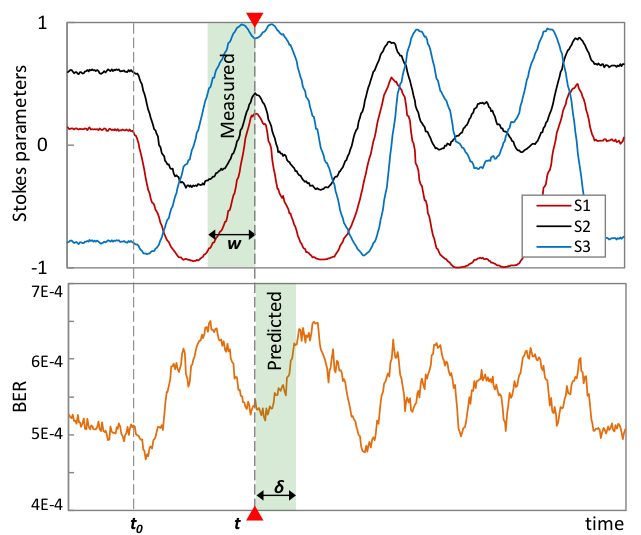
\includegraphics[width=0.6\linewidth]{img/previousWork_w_d.png}
    \caption{Prediction of the Bit Error Rate (BER) based on the state of polarization (SOP) with recording and prediction windows (w and d)}
    \label{previous}
\end{figure}
% %\vspace*{-15pt}

% quick presentation of previous work
A research paper that studies and builds this kind of model has been presented in \cite{Benham}. In this paper, the authors show that a very simple model can be trained to predict the BER of a light path in the event of a physical disturbance of a single fiber. Our work will be based on the results of the research paper. We aim to build a new prediction model, that uses kernel methods to predict the value of the error rate.

% sections organization
We will first present the previous work performed in \cite{Benham} in terms of data preprocessing, model fitting and results. We will then show how we can replicate the same model and results. After that, new models that improve the results of the prediction will be proposed and final comparison table will be built.



\section{Previous Work}


% present paper and authors
% present dataset 
In the study from the reference research paper \cite{Benham}, the authors performed an important preprocessing work on the original dataset. 
The data set consists of the measurement of 3 variables of an optical fiber communication channel which are called State of Polarization (SOP), and the bit error rate measurement (BER). Those variables are gathered during periods of 4 seconds, during which a robotic arm that holds the optic fiber performs a physical action like rotation and or translation. The values are stored at a rate of 4000 values per second (1 value every 0.25ms) and there are a total of 360 experiments that last 4 seconds each. The SOP variables are constrained to form a vector that lives in the unit sphere.

%present preprocessing and model
In the previous work, the researchers built a prediction model of the error rate based on 6 variables gathered in time windows of $w$ ms. Those variables consisted in :
\begin{itemize}
    \item the final value in the time window (at time t) of the 3 SOP variables
    \item the trends of each SOP within the time window [t-w,t]
\end{itemize}

The prediction goal was the BER value at $\delta$ ms after the last instance of the time windows. The values of the time window and the $\delta$ tested where between 10 and 300ms.
The variables and the BER where then discretized into p and q segments of equal length respectively. Then a Naive Bayes model was trained. Model accuracy was computed by the relative prediction error (RPE), defined as (predictedBER-realBER)/realBER), a measure that ranged from 3\% to 12\% in the reference paper's results. Different were models trained for different values of the observation window $w$ and the prediction window $\delta$. Their results are shown in the following figures:


\begin{figure}[H]
\minipage{0.5\textwidth}%
  \centering
    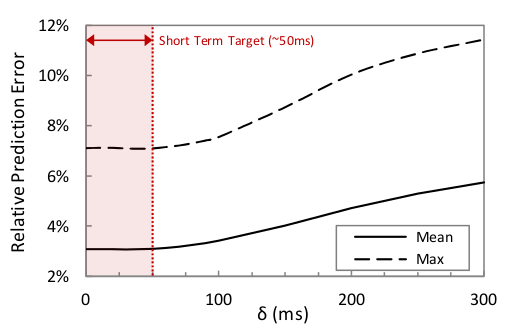
\includegraphics[width=0.9\linewidth]{img/previous_model1.png}
\endminipage\hfill
\minipage{0.5\textwidth}%
  \centering
    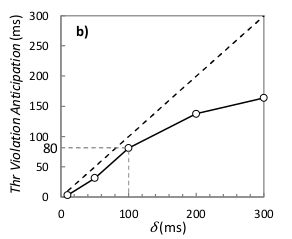
\includegraphics[width=0.9\linewidth]{img/previous_model2.png}
\endminipage\label{previous1}\caption{Plot of the Relative Prediction Error (RPE) of the models from the reference paper}
\end{figure}



% %\vspace*{-15pt}
\begin{figure}[H]
    \centering
    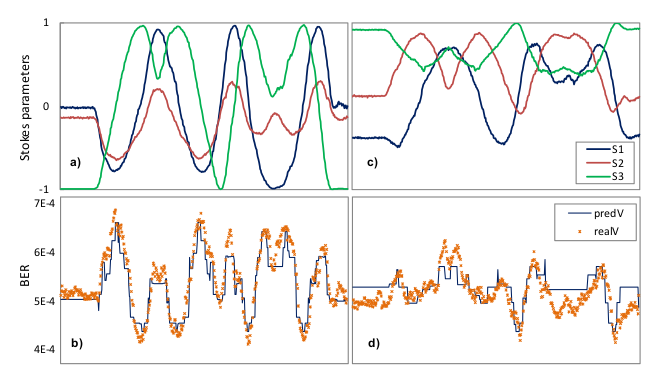
\includegraphics[width=0.8\linewidth]{img/previousWork_prediction.png}
    \caption{Prediction of the BER with a Naive Bayes algorithm from the previous work}
    \label{previous2}
\end{figure}
% %\vspace*{-15pt}




\section{Replicating previous work}

In order to improve the predictive model, we need to replicate the reference paper's model to be able to completely compare new models accuracy, using the same measure, the mean relative prediction error. In this section we will explain how we replicated the data preprocessing, the model fitting and the model selection performed in the reference paper.

% In order to compare our Kernel model with proposed solution by previous researchers, we decided to first replicate the experiment and recorded Mean Average Percentage Error (MAPE)
% for Naive Bayes and SVM (with rbf kernel and default parameters).\\\\

\subsection{Data Preprocessing}

First we need to perform same pre-processing as it was done before. We take the original data and for each window and $\delta$ we downsample it and then discretize. Discretization is done in order to transform regression problem to classification one. We map each predictable variable $\hat{y}$ to a respective uniformly constructed interval. And take the median of this interval as a class. This transformation is necessary because we are solving the classification problem, but we want to measure Mean Average Percentage Error, instead of classification accuracy. This is done by comparing real measure of $y$ with predicted $\hat{y}$, where $\hat{y}$ is a median of a predicted interval. The features that are used in training and testing are $x_1,x_2,x_3,sx_1,sx_2,sx_3$, where $x_i$ are coordinates in unit sphere, $sx_i$ are slopes of $x_i$, $i \in [1,3]$.\\\\

\subsection{Naive Bayes model}

To replicate the previous work, we fit a Naive Bayes model to the data. We train different Naive Bayes models for various window sizes and $\delta$-s. We also compute the same error measure as the reference paper. We record both the Mean Average Percentage Error (MEPA) and the maximum percentage error found when predicting over the testing dataset. The results can be seen in the table \ref{tab:results_prev}

\subsection{Results}

\begin{table}[!h]
\centering
\caption{Previous work results}
\label{tab:results_prev}
\begin{tabular}{rrrrr}
  \hline
 & W & $\delta$ & Naive Bayes MAPE & SVM MAPE \\ 
  \hline
1 & 10 & 10 & 0.04508 & 0.04317 \\ 
  2 & 10 & 50 & 0.04513 & 0.04331 \\ 
  3 & 10 & 100 & 0.04462 & 0.04318 \\ 
  4 & 10 & 200 & 0.04380 & 0.04345 \\ 
  5 & 10 & 300 & 0.04345 & 0.04342 \\ 
  6 & 20 & 10 & 0.04489 & 0.04322 \\ 
  7 & 20 & 50 & 0.04498 & 0.04328 \\ 
  8 & 20 & 100 & 0.04446 & 0.04340 \\ 
  9 & 20 & 200 & 0.04387 & 0.04335 \\ 
  10 & 20 & 300 & 0.04373 & 0.04345 \\ 
  11 & 30 & 10 & 0.04486 & 0.04322 \\ 
  12 & 30 & 50 & 0.04517 & 0.04349 \\ 
  13 & 30 & 100 & 0.04465 & 0.04337 \\ 
  14 & 30 & 200 & 0.04382 & 0.04328 \\ 
  15 & 30 & 300 & 0.04366 & 0.04345 \\ 
  16 & 40 & 10 & 0.04499 & 0.04327 \\ 
  17 & 40 & 50 & 0.04509 & 0.04329 \\ 
  18 & 40 & 100 & 0.04467 & 0.04311 \\ 
  19 & 40 & 200 & 0.04387 & 0.04328 \\ 
  20 & 40 & 300 & 0.04365 & 0.04343 \\ 
  21 & 50 & 10 & 0.04507 & 0.04328 \\ 
  22 & 50 & 50 & 0.04491 & 0.04350 \\ 
  23 & 50 & 100 & 0.04463 & 0.04323 \\ 
  24 & 50 & 200 & 0.04371 & 0.04342 \\ 
  25 & 50 & 300 & 0.04372 & 0.04323 \\ 
  26 & 100 & 10 & 0.04512 & 0.04338 \\ 
  27 & 100 & 50 & 0.04496 & 0.04340 \\ 
  28 & 100 & 100 & 0.04464 & 0.04340 \\ 
  29 & 100 & 200 & 0.04388 & 0.04335 \\ 
  30 & 100 & 300 & 0.04389 & 0.04333 \\ 
  31 & 150 & 10 & 0.04527 & 0.04341 \\ 
  32 & 150 & 50 & 0.04515 & 0.04338 \\ 
  33 & 150 & 100 & 0.04448 & 0.04337 \\ 
  34 & 150 & 200 & 0.04391 & 0.04362 \\ 
  35 & 150 & 300 & 0.04388 & 0.04338 \\ 
  36 & 200 & 10 & 0.04539 & 0.04343 \\ 
  37 & 200 & 50 & 0.04493 & 0.04311 \\ 
  38 & 200 & 100 & 0.04473 & 0.04343 \\ 
  39 & 200 & 200 & 0.04388 & 0.04345 \\ 
  40 & 200 & 300 & 0.04380 & 0.04343 \\ 
   \hline
\end{tabular}
\end{table}



These are the results of the error measures obtained when replicating the previous work.

\begin{figure}[H]
    \centering
    \includegraphics[width=0.8\linewidth]{img/previousWor_RPE_plot.png}
    \caption{Prediction error for different prediction windows $\delta$ for a fixed observation window w}
    \label{previous2}
\end{figure}


\section{Improvements}

In this section we are going to apply a different model, an SVM, to improve the results of the previous model.

\subsection{SVM model}

Preprocessing of the data...(discretization, lagged windows, PCA of the lagged features, removing one SOP var as it is constrained)

Model, HP and model selection...


Results...

As we can see in the table \ref{tab:results_prev} the results of SVM are slightly better than results of Naive Bayes method. Which mean it will be possible to improve the results slightly with right hyper parameters.

In order to improve the results, i.e. test error, we will apply support vector machines on both same data and/or transformed in another way. Perform cross validation to select the best hyper parameters and rerun the model on several window sizes and $\delta$=100ms, since that was the proposed long-term model of previous researchers. By this we will be able to compare our solution with previous one.

\subsection{SVM for regression}

Preprocessing...

Model construction, kernels and model selection...

\subsection{RVM for regression}

Preprocessing...

Model construction, kernels and model selection...




\section{Results}

This section summarizes the results obtained with different models.

Table of best models of each kind...

Combined plot of Predicted error for different d for a fixed w...


\section{Conclusion}



\begin{thebibliography}{9}
\bibitem{Benham} 
B. Shariati, F. Boitier , M. Ruiz , P. Layec , and L. Velasco.
\textit{Autonomic Transmission Through pre-FEC BER Degradation Prediction Based on SOP Monitoring,}. 
European Conference on Optical Communication, 2018.
 
\end{thebibliography}




% \section{Predictive Model}

% Different alternatives are proposed for this project:
% \begin{itemize}
% \item Classification model: a similar discretization could be performed on the value of the BER. For the variables, we could then use all the values of each SOP during a specific time window, with a specific granularity (for example: one value at each ms during a time window of 10 ms). In that case, an SVM model could be trained. One of the interesting points of this approach is to choose a powerful kernel that yields good results. We could also use a BER value from $t+\delta$ for a time window [t-w,t].
% \item Regression model: we could avoid doing a discretization of the values and train a regression model using SVM for regression. We could also use a BER value from $t+\delta$ for a time window [t-w,t].
% \item Time series prediction: we will base our work on a paper by  Müller, Vapnik et. al, which explains how to use support vector machines for time series prediction. 
% \end{itemize}






% \section{Preprocessing}



% The preprocessing will consist in the following steps:
% \begin{enumerate}
% \item Import data from multiple csv files into one data frame, selecting the columns related to the SOP and the error (BER)
% \item Downsample the data from 1 value each 0.25ms to some reasonable value like 1 value each 1ms, 5ms or 10ms. We will consider also applying a moving average smoothing procedure to reduce noise, specially in the BER value.
% \item Transform the dataset from 3 variables (SOP values) and one target (BER) to a dataset that contains w values from time t-w to time t for each SOP variables and for the BER, plus a value for the BER at time t+d.  We will select the values of w and d according to previous work,  applicability to the real case scenario where this model could be implemented and also suitability of the predictive models.
% \end{enumerate}

% \subsection{Importing data from csv files}

% Each csv file corresponds to a 4 second experiment. The data has been imported into a data frame, by selection the values of the x1,x2 and x3 SOP variables and the BER. The dataframe contains also an indication of the origin file. This will used when computing the lagged values of each SOP variables, since we won't be merging values from one experiment (one csv file) with values from another one.

% \subsection{Downsampling and Moving average}



% \begin{figure}[H]
% \minipage{0.5\textwidth}%
%   \centering
%     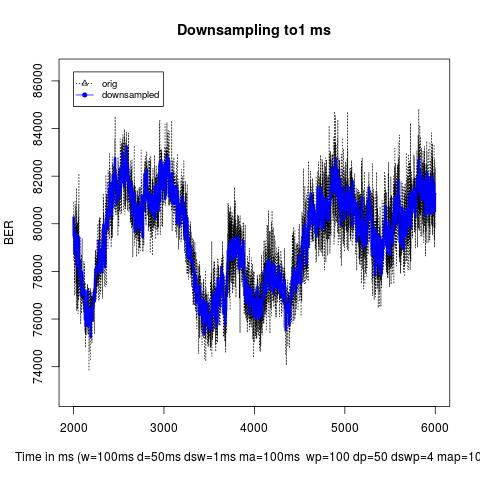
\includegraphics[width=0.9\linewidth]{img/downsampling_Time_in_ms_(w_100ms_d_50ms_dsw_1ms_ma_100ms__wp_100_dp_50_dswp_4_map_100).jpeg}
% \endminipage\hfill
% \minipage{0.5\textwidth}%
%   \centering
%     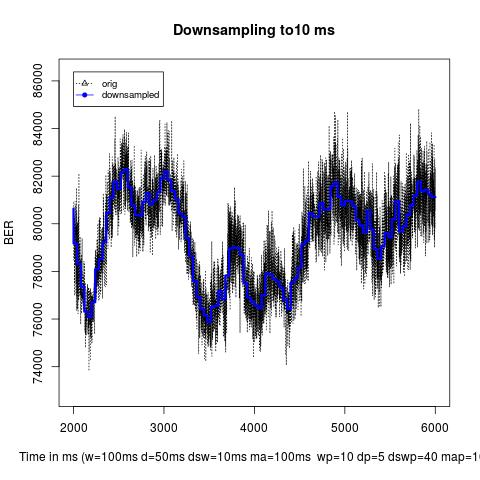
\includegraphics[width=0.9\linewidth]{img/downsampling_Time_in_ms_(w_100ms_d_50ms_dsw_10ms_ma_100ms__wp_10_dp_5_dswp_40_map_10).jpeg}
% \endminipage\vfill
% \minipage{0.5\textwidth}%
%   \centering
%     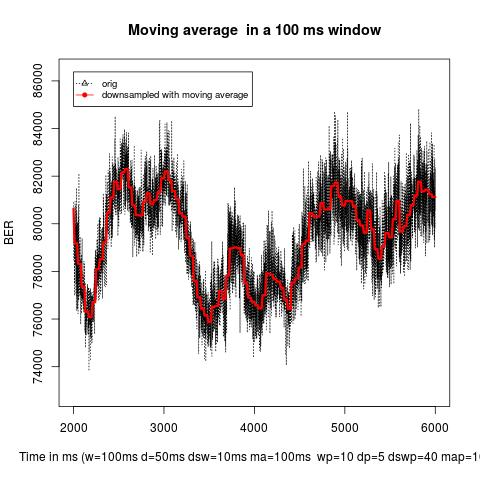
\includegraphics[width=0.9\linewidth]{img/ma_Time_in_ms_(w_100ms_d_50ms_dsw_10ms_ma_100ms__wp_10_dp_5_dswp_40_map_10).jpeg}
% \endminipage\hfill
% \minipage{0.5\textwidth}%
%   \centering
%     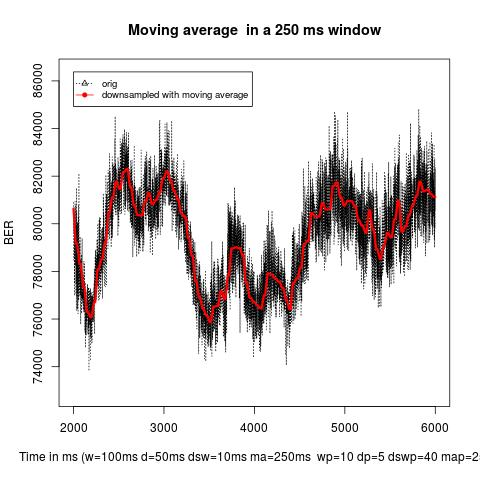
\includegraphics[width=0.9\linewidth]{img/ma_Time_in_ms_(w_100ms_d_50ms_dsw_10ms_ma_250ms__wp_10_dp_5_dswp_40_map_25).jpeg}
% \endminipage

% \caption{Ploting different downsampling rates and moving averages combined}
% \end{figure}

% We see that the downsampling to 10ms rate removes the a good quantity of noise in the target variable but even if it maintains the major trend and eliminates small noise it also erases some important fluctuation we want to capture. 

% \begin{figure}[H]
%     \centering
%     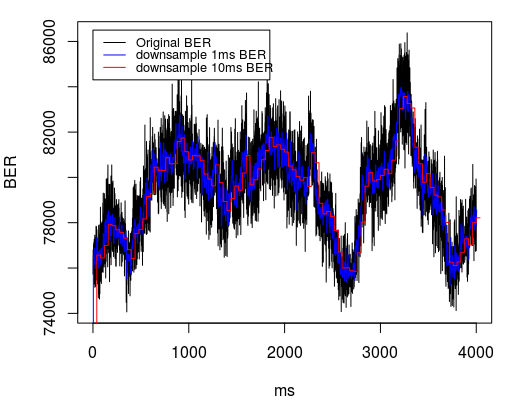
\includegraphics[width=0.8\linewidth]{img/donwsamplingBER.png}
%     \caption{Different downsampling applied to the BER signal}
%     \label{previous2}
% \end{figure}


% A second plot with the values of the SOP variables shows that a downsampling to 1ms rate is the best choice.

% \subsection{Transforming the dataset }
%  We will transform the data set into a sequence of time series values for each SOP variable and the BER value in a time window from t-w to t. We will also add the future BER value in an instance t+d.
%  The selected values that we will test the models on will be:
%  \begin{itemize}
%      \item w=50,100,200,500 and 1000ms 
%      \item d=50,100,200ms
%  \end{itemize}
 
% \section{Predictive Models}

% \subsection{Model selection}

% We will train different models with different hyperparameters for different parameters of the prediction (w,d). We will perform model selection by cross-validation based on the Root Mean Squared Error (RMSE) averaged over the different folds.
% Once the model has been selected, it is trained again with all the training data.
% The comparisons of different models will be performed agains this averaged RMSE. We will also try to compared the new models to the model used in the previous work, for which we will have to transform our predicted output to the discretized classes they used in this previous study.

% \subsection{Types of models}

% We will filt SVM and RVM for regression models to our data set to predict the value of the BER at a future time t+d. For such task we will train those types of models with several different kernels (Gaussian RBF, Polynomial, Laplace, String) with different values of their hyperparameters.

% \subsection{Training procedure}

% We sample the dataset into a training and testing subset, and then we will divide the training set into k subsets to be able to apply a cross-validation procedure.
% We limit the complexity of the model to adjust it to our computation resources (training models for more than a couple of hours is prohibitive). Since the after applying the kernel transformation, the complexity of the model becomes a function of the number of samples in the original space, we limit the number of samples that we feed to each model according to the number of features (we need n < d, with n number of samples and d number of features).
% % Also, since the RVM does not minimize a convex function, it can get stuck in local optima. For this reason we need to train each model and hyperparameter setup several times. We can also augment the number of execution of the training of a specific model by using this limitation on the input size to our advantage,  and use it to train the same specific model for different training datasets. 

% \section{Results}

% \begin{table}[H]
% \centering
% \adjustbox{maxheight=\dimexpr\textheight-5.9cm\relax, max width=\textwidth, center}{
% \begin{tabular}{ccccccccccc}
%   \hline
%  & Algorithm & Kernel & e & C & sigma & w & d & downsampling & moving avg & RMSE \\ 
%  &  &  &  &  &  & (ms) & (ms)  & (ms) & (ms) &  \\ 
%   \hline
%   %svm.rbf__n_1500_sigma_1e-07_e_0.1_C_100_dim__1168___4004_csv_small5_w1000ms_d100ms_wp400_dp40_dsw10_maw250_8.18secs_rmse_230.889
% 1 & SVM & RBF  & 0.1 & 100  & 1e-07 & 1000 & 100  & 10  & 250  & 230.89  \\
% %svm.rbf__n_1500_sigma_1e-06_e_0.1_C_100_dim__1168___4004_csv_small5_w1000ms_d100ms_wp400_dp40_dsw10_maw250_6.78secs_rmse_144.574
% 2 & SVM & RBF  & 0.1 & 1000  & 1e-06 & 500 & 100  & 1  & 10  & 144.57  \\ 
% %rvm.rbf__n_1500_sigma_1e-11_dim__1168___4004_csv_small5_w1000ms_d100ms_wp400_dp40_dsw10_maw250_53.07secs_rmse_240.591
% 3 & RVM & RBF  &  &  & 1e-11 & 1000 & 100  & 10  & 250  & 240.59  \\
% %svm.rbf__n_1500_sigma_1e-05_e_0.1_C_1000_dim__1704___2004_csv_small5_w500ms_d100ms_wp2000_dp400_dsw1_maw10_12.82secs_rmse_3674.661
% 4 & SVM & RBF  & 0.1 & 1000  & 1e-05 & 500 & 100  & 1  & 10  & 3674.66  \\
%  \hline
% \end{tabular}
% } \caption{Model selection results}
% \end{table}




% \begin{figure}[H]
% \minipage{0.5\textwidth}%
%   \centering
%     \includegraphics[width=0.7\linewidth]{img/model1.jpeg}
% \endminipage\hfill
% \minipage{0.5\textwidth}%
%   \centering
%     \includegraphics[width=0.9\linewidth]{img/model2_test_sop.jpeg}
% \endminipage
% \caption{Model 2 prediction over the validation set}
% \end{figure}

% \begin{figure}[H]
%     \centering
%     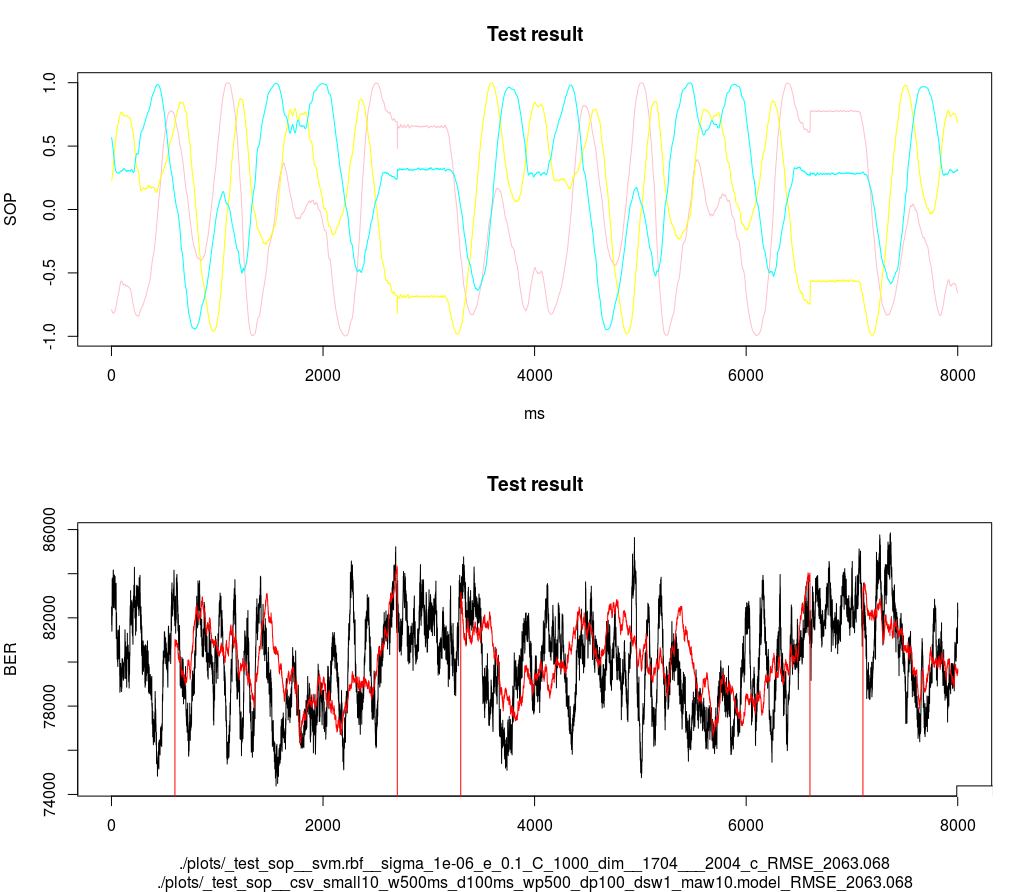
\includegraphics[width=0.7\linewidth]{img/Prediction_svm_se-6_0_1e_1000e_dsw=1_w500_d100.png}
%     \caption{Model 2 prediction over the test set}
%     \label{model2res}
% \end{figure}



% \begin{figure}[H]
%     \centering
% \includegraphics[width=0.7\linewidth]{img/model4_test_sop__svm_rbf__n_1500_sigma_1e-05_e_0_1_C_1000_dim__1704___2004_csv_small5_w500ms_d100ms_wp2000_dp400_dsw1_maw10_model_RMSE_2382.jpeg}
% \caption{Model 4 prediction over the validation set}
%     \label{model2res}
% \end{figure}



% \begin{figure}[H]
% \minipage{0.5\textwidth}%
%   \centering
%     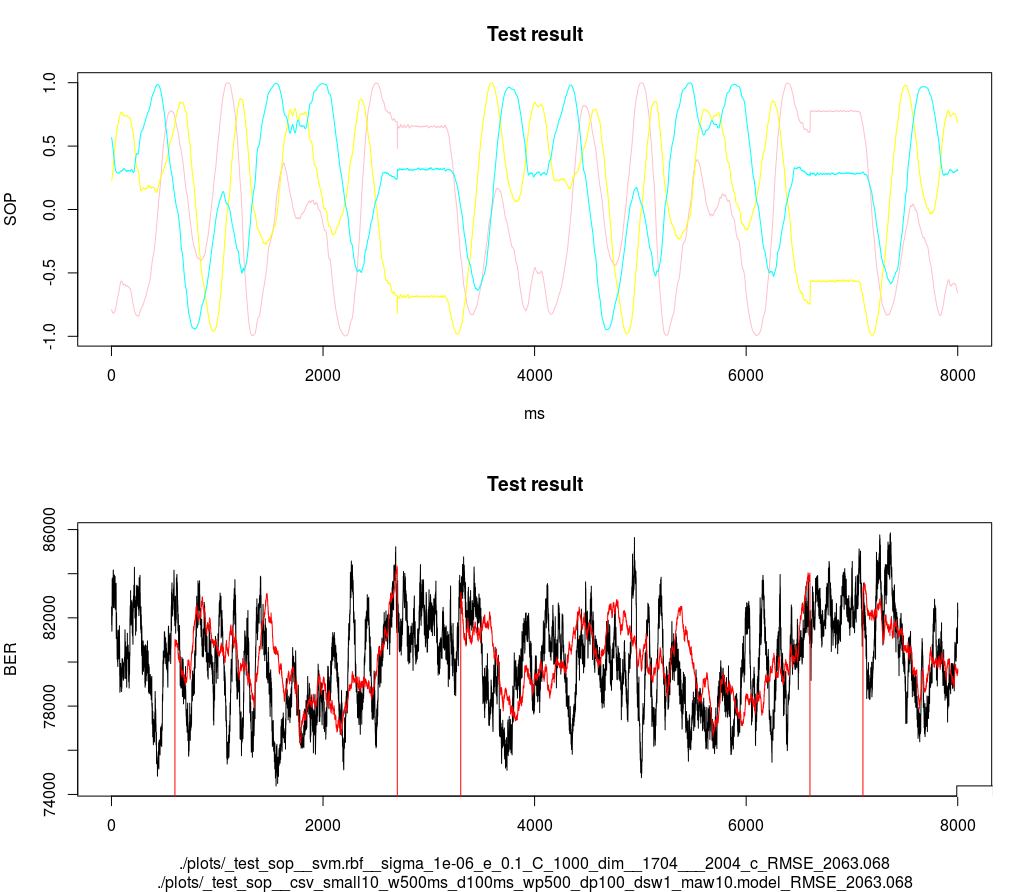
\includegraphics[width=1\linewidth]{img/Prediction_svm_se-6_0_1e_1000e_dsw=1_w500_d100.png}
%     \caption{Model 2 prediction over the test set}
% \endminipage\hfill
% \minipage{0.5\textwidth}%
%   \centering
%     \includegraphics[width=0.85\linewidth]{img/model4_test_sop__svm_rbf__n_1500_sigma_1e-05_e_0_1_C_1000_dim__1704___2004_csv_small5_w500ms_d100ms_wp2000_dp400_dsw1_maw10_model_RMSE_2382.jpeg}
% \caption{Model 4 prediction over the validation set}
% \endminipage
% \end{figure}

% \section{Conclusion}

% The focus of this project has been twofold, apply a kernelized machine learning algorithm to a previous work, and study the performance of different kernels for the task of time series prediction.




\end{document}





% %\vspace*{-15pt}
% \begin{figure}[H]
%     \centering
%     \includegraphics[width=0.8\linewidth]{img/Altmann.png}
%     \caption{Optimized parameters for the Altmann function for different initial values ranging from 0.01 to 50 in logarithmic increments}
%     \label{fig:altmann}
% \end{figure}
% %\vspace*{-15pt}



% \begin{figure}[H]
% \minipage{0.5\textwidth}%
%   \centering
%     \includegraphics[width=0.9\linewidth]{img/csn_task2_comm3200_walktrap.png}
%     \caption{Financial ratio related community}\label{com02}
% \endminipage\hfill
% \minipage{0.5\textwidth}%
%   \centering
%     \includegraphics[width=0.9\linewidth]{img/csn_task2_comm3202_walktrap.png}
%     \caption{Credit card related community}\label{com03}
% \endminipage
% \end{figure}\caption{Communities found with the Walktrap community detection algorithm}




